\section{Introduction}

The aim of this project was to develop an application that would allow users to write using a robot arm. Thus, we decided to focus on making our application user-friendly and performant.\\
To do so, we implemented 2 modes. The first one allows us to use gestures to write letters by letters. The second mode is designed so the robot's arm follows the finger of the user. \\

The selection of mode is done as the start of the application but can also be done at every moment while using the application through \textit{master gestures}.

\begin{figure}[H]
	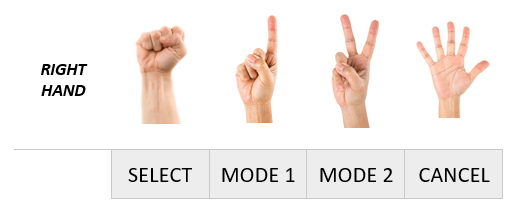
\includegraphics{mode_selection}
	\centering
	\caption{Mode selection - set of gestures}
	\label{fig:mode}
\end{figure}
